% 贝赛尔函数
% 贝赛尔方程|贝赛尔函数|汉克尔函数|修正贝赛尔函数

贝赛尔方程为% 链接未完成
\begin{equation}
x^2 \dv[2]{y}{x} + x\dv{y}{x} + (x^2 - \alpha ^2)y = 0
\end{equation}
其中 $\alpha$ 叫做阶数. 两个线性无关的解分别是\textbf{第一类贝赛尔函数} $J_\alpha(x)$ 和\textbf{第二类贝赛尔函数} $Y_\alpha(x)$. 这里只讨论 $x > 0$ 且 $\alpha$ 为整数或半整数的情况.

\begin{figure}[ht]
\centering
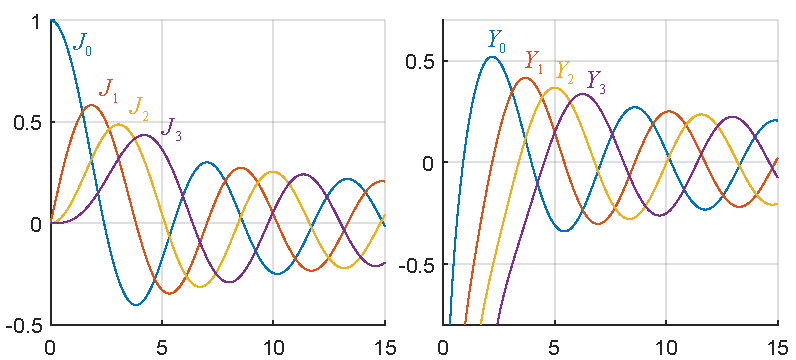
\includegraphics[width=13cm]{./figures/Bessel_1.pdf}
\caption{第一类和第二类贝赛尔函数} \label{Bessel_fig1}
\end{figure}

$J_\alpha(x)$ 的级数形式为
\begin{equation}
J_\alpha(x) = \sum_{m=0}^\infty \frac{(-1)^m}{m!\Gamma(m+\alpha+1)} \qty(\frac x2)^{2m+\alpha}
\end{equation}
其中使用了 $\Gamma$ 函数\upref{Gamma}. $Y_\alpha(x)$ 可以通过 $J_\alpha(x)$ 来定义
\begin{equation}
Y_\alpha(x) = \frac{J_\alpha(x)\cos\alpha\pi - J_{-\alpha}(x)}{\sin\alpha\pi}
\end{equation}

\subsection{汉克尔函数}
贝赛尔方程的两个线性无关解也可以用第一类和第二类汉克尔函数来表示\footnote{可类比欧拉公式 $\exp(\pm\I x) = \cos x \pm \I\sin x$ (\autoref{CExp_eq2}~\upref{CExp}).}
\begin{equation}
H_\alpha ^{(1)}(x) = J_\alpha(x) + \I Y_\alpha(x)
\qquad
H_\alpha ^{(2)}(x) = J_\alpha(x) - \I Y_\alpha(x)
\end{equation}

\subsection{常用性质}
令 $Z$ 为 $J, Y, H^{(1)}, H^{(2)}$ 的任意一种, 则
\begin{equation}
Z_{-\alpha}(x) = (-1)^\alpha Z_\alpha(x)
\end{equation}
递推关系
\begin{equation}
\frac{2\alpha}{x} Z_\alpha(x) = Z_{\alpha -1}(x) + Z_{\alpha+1}(x)
\end{equation}
一阶导数
\begin{equation}
\dv{Z_\alpha}{x} = \frac12 [Z_{\alpha  - 1}(x) - Z_{\alpha +1}(x)]
\end{equation}
正交关系
\begin{equation}
\int_0^1 x J_\alpha (u_{\alpha ,m} x) J_\alpha (u_{\alpha ,n} x) \dd{x} = \frac{\delta_{m,n}}{2}[J_{\alpha + 1} (u_{\alpha ,m})]^2
\end{equation}
其中 $u_{\alpha, m}$ 是 $J_\alpha(x)$ 的第 $m$ 个根.

\subsection{修正贝赛尔函数}
修正贝赛尔方程为
\begin{equation}
x^2 \dv[2]{y}{x} + x \dv{y}{x} - (x^2 + \alpha ^2)y = 0
\end{equation}
其解为两个\textbf{修正贝赛尔函数(Modified Bessel Function)},第一类为 $I_\alpha(x)$,  第二类为 $K_\alpha(x)$,  与贝赛尔函数的关系为
\begin{equation}
I_\alpha(x) = \I^{-\alpha} J_\alpha(\I x)
\qquad
K_\alpha(x) = \frac{\pi}{2} \I^{\alpha  + 1} H_\alpha ^{(1)}(\I x)
\end{equation}

